\section{Durchführung}
\label{sec:Durchführung}
In Der Versuchsdurchführung gibt es zwei teile, einmal das aufnehmen der Messwerte für eine Schar von fünf Kennlinien, 
mit dessen hilfe die Settigungsströme ermitelt und das Langmuir-Schottky’sche Raumladungsgesetz bestimmt werden kann.
\subsection{Bestimung der Kennlinien}
\label{sec:1}
Es soll eine schaar von Fünf verschiedenen Kennlinien dargestellt werden, also für Jewails fünf verschiedene 
Heitzspannungen. Die Schaltung wird gemäß \autoref{fig:3} aufgebaut, welche auch in \autoref{fig:5} dargestellt ist.
Ganz vorne im Bild ist die Vakuum-Diode abgebildet. Diese ist an einen Heitsspannungs und Stromgenerator links angeschlossen.
Wird dort eine Spannung eingestellt, beginnt die Kathode und damit das Wolfram zu glühen und es treten Elektronen aus.
 Außerdem wird 
an die Diode mit einer weiteren Spannnungsquelle rechts im Bild eine Spannung angelegt, die sogenannte "Absaugspannung". diese wird 
dann kontinuirlich in kleinen Schritten erhöht und wird jeweils gegen den gemessene Absaugstrom aufgetragen.
\begin{figure}[H]
    \centering
        \centering
        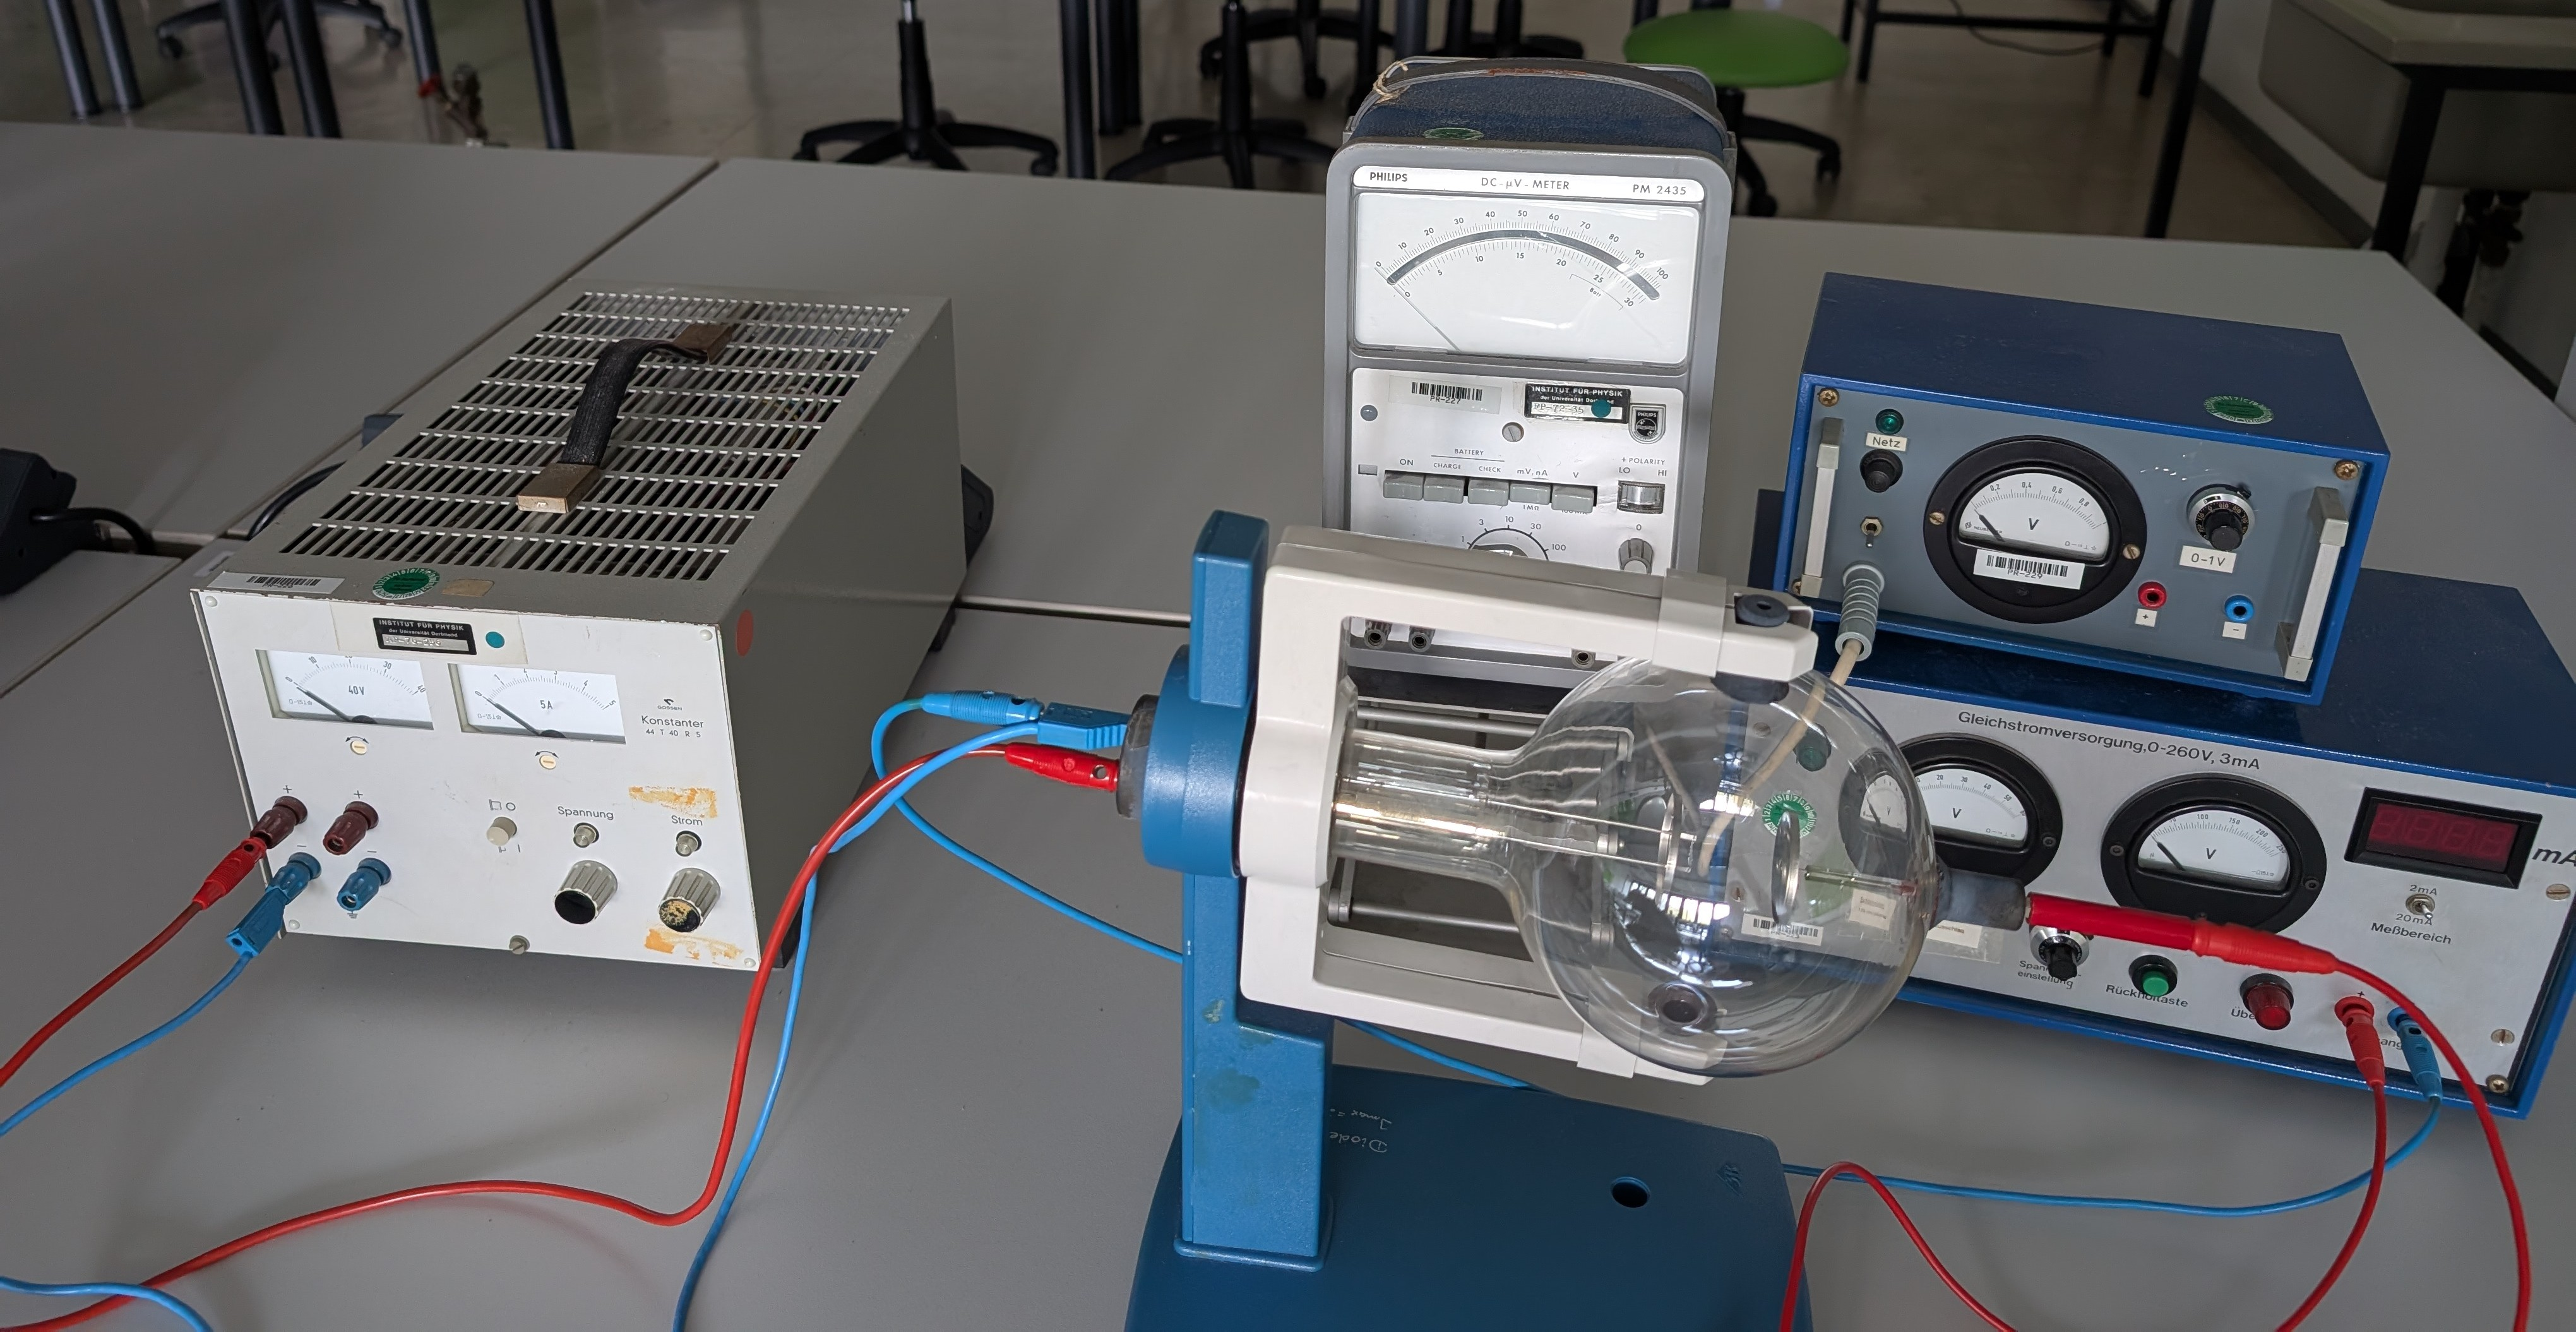
\includegraphics[width=\textwidth]{Bilder/2.jpg}
        \caption{Aufbau zur messung der Kennlinien.}
    \hfill
    \label{fig:4}
\end{figure}

\subsection{Das Anlaufstromgebiet}
Um den bereich des Anlaufstromgebiets festzulegen wird die in abbildung \autoref{fig:5} abgebildete Schaltung aufgebaut. Sie unterscheidet sich 
darin von der Schaltung aus \autoref{sec:1}, dass diesmal ein anders herum gepoltes kleineres$\left(1 - 2\unit{\volt}\right)$ Gegenfeld an die Vakuum Diode angeschlossen wird.
Nun wird eine Heitzspannung eingestellt und die Spannung des Gegenfeldes wird von null bis Zehn Volt in 0.5er schritten erhöht und der Anlaufstrom wird abgelesen.
\begin{figure}[H]
    \centering
        \centering
        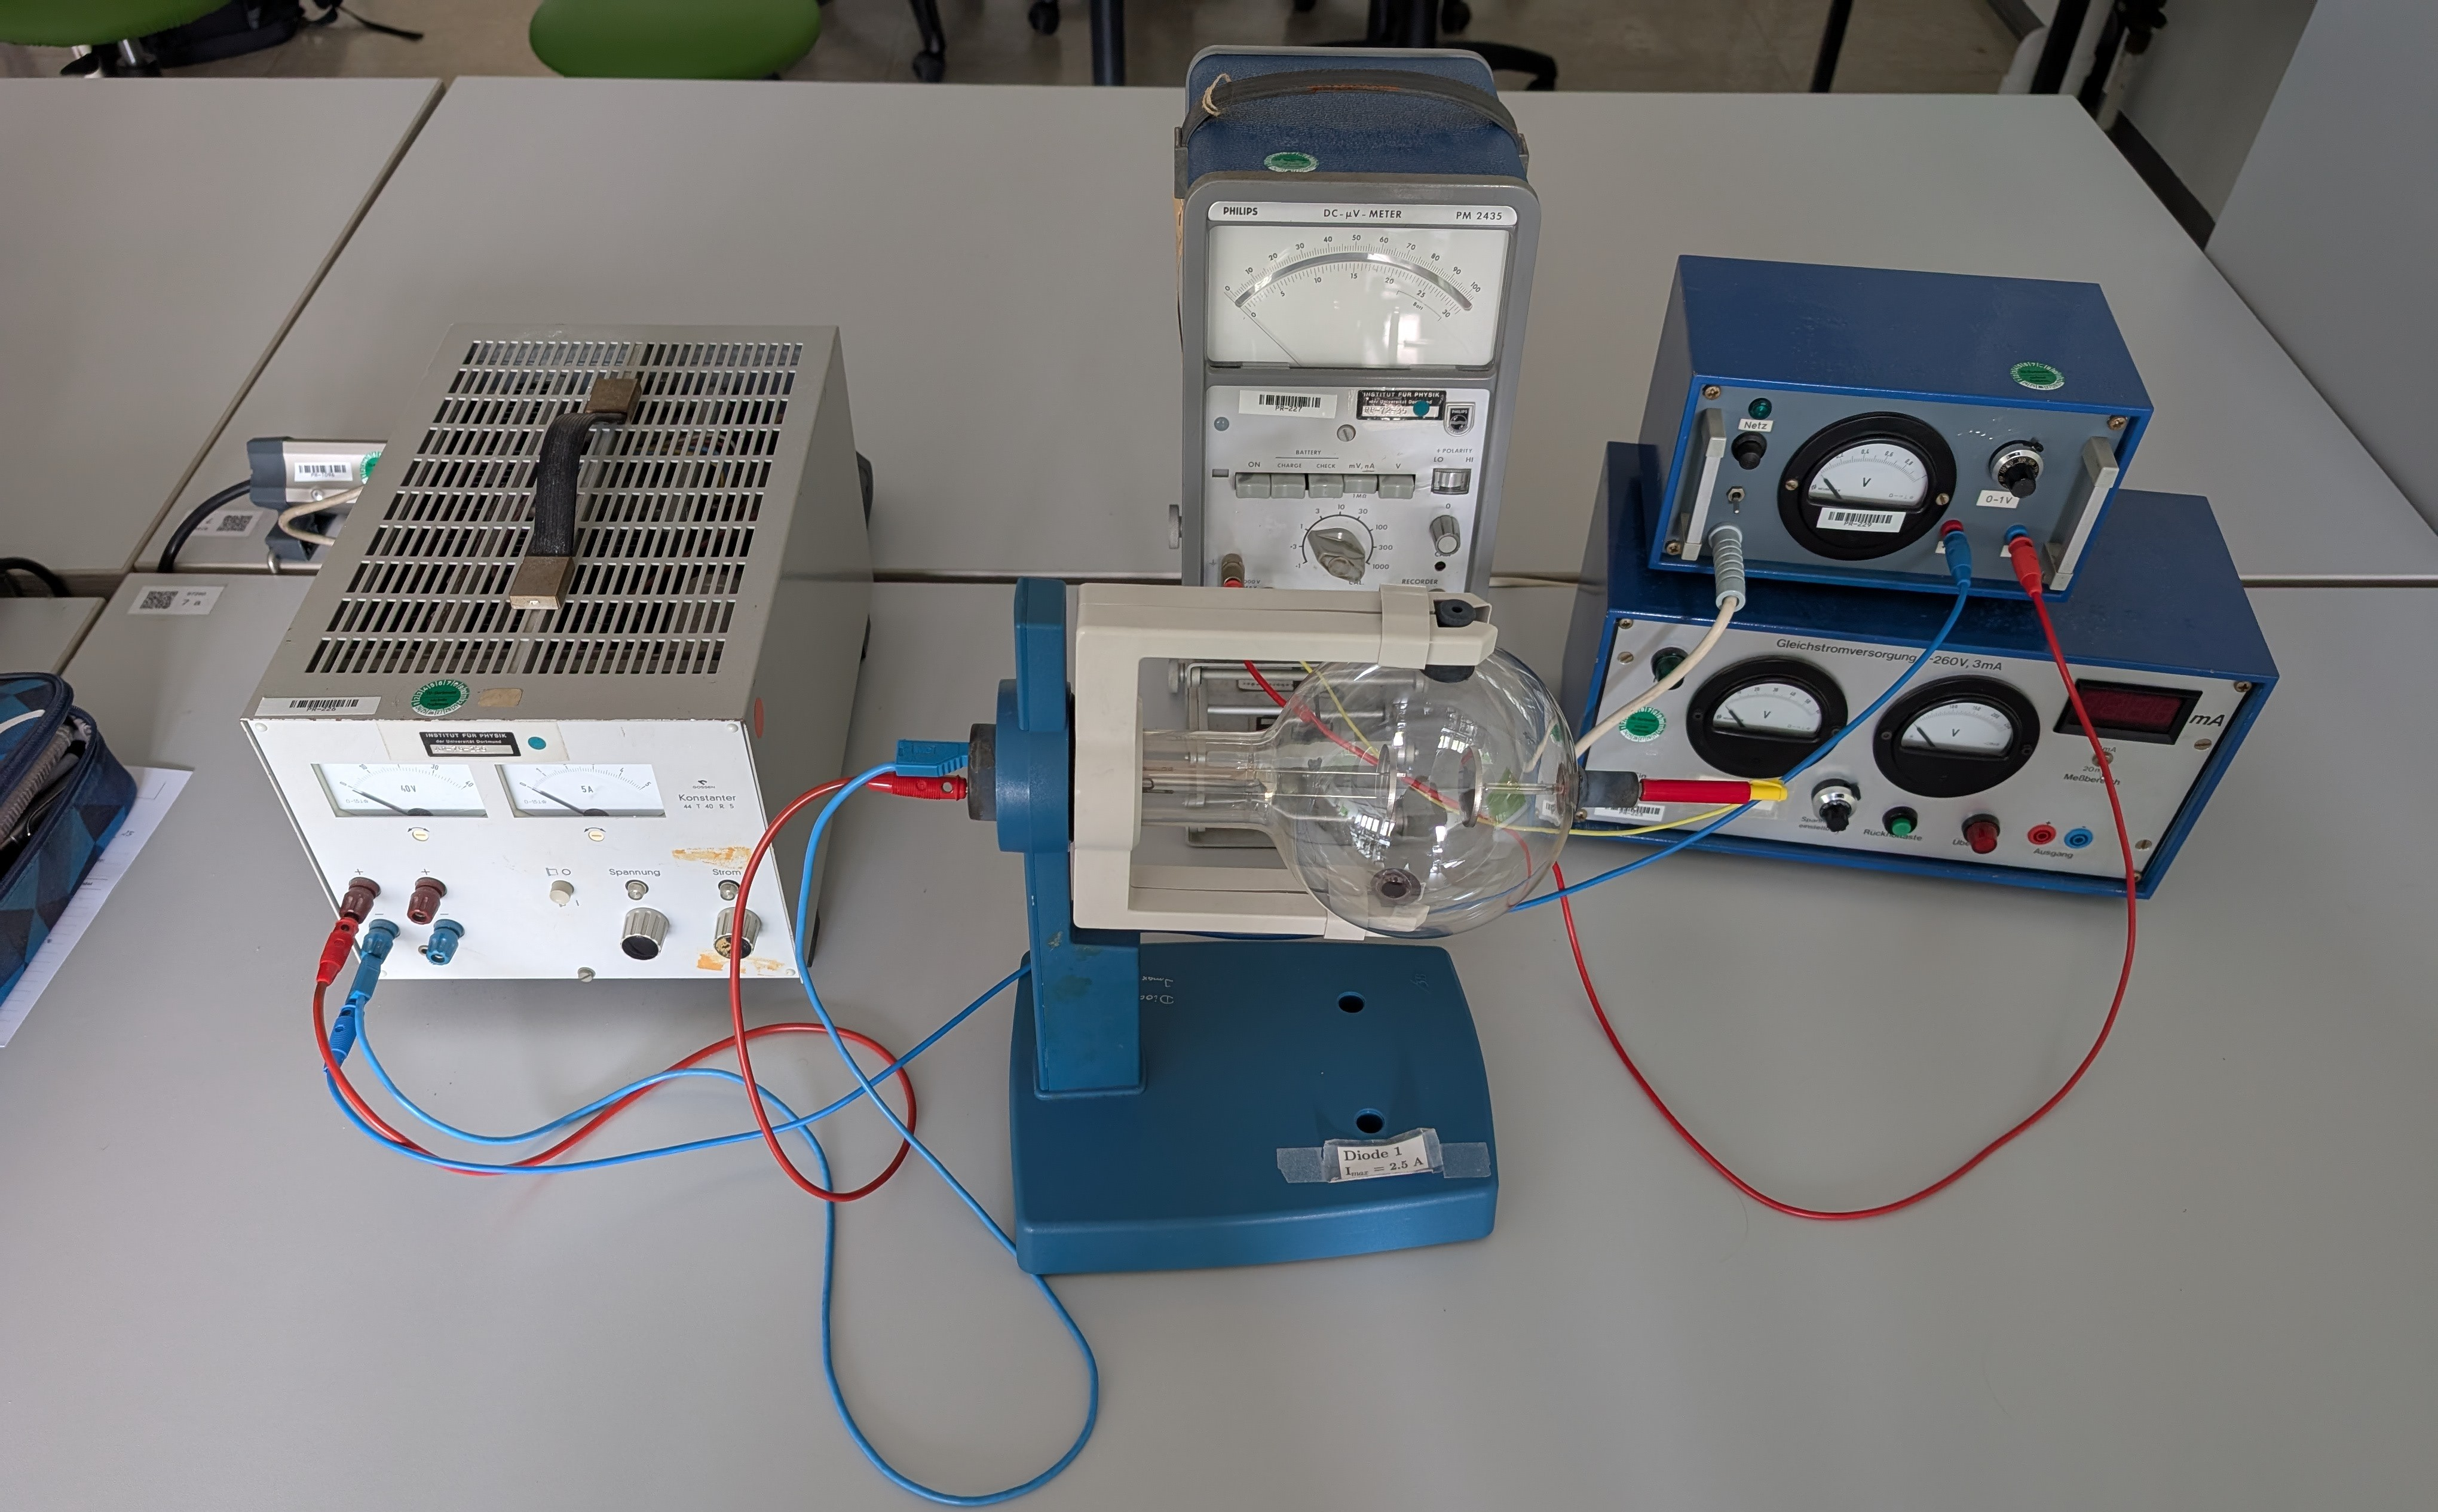
\includegraphics[width=\textwidth]{Bilder/1.jpg}
        \caption{Schaltung zur messung des Anlaufstromgebiets}
    \hfill
    \label{fig:5}
\end{figure}
\begin{figure}[H]
    \centering
        \centering
        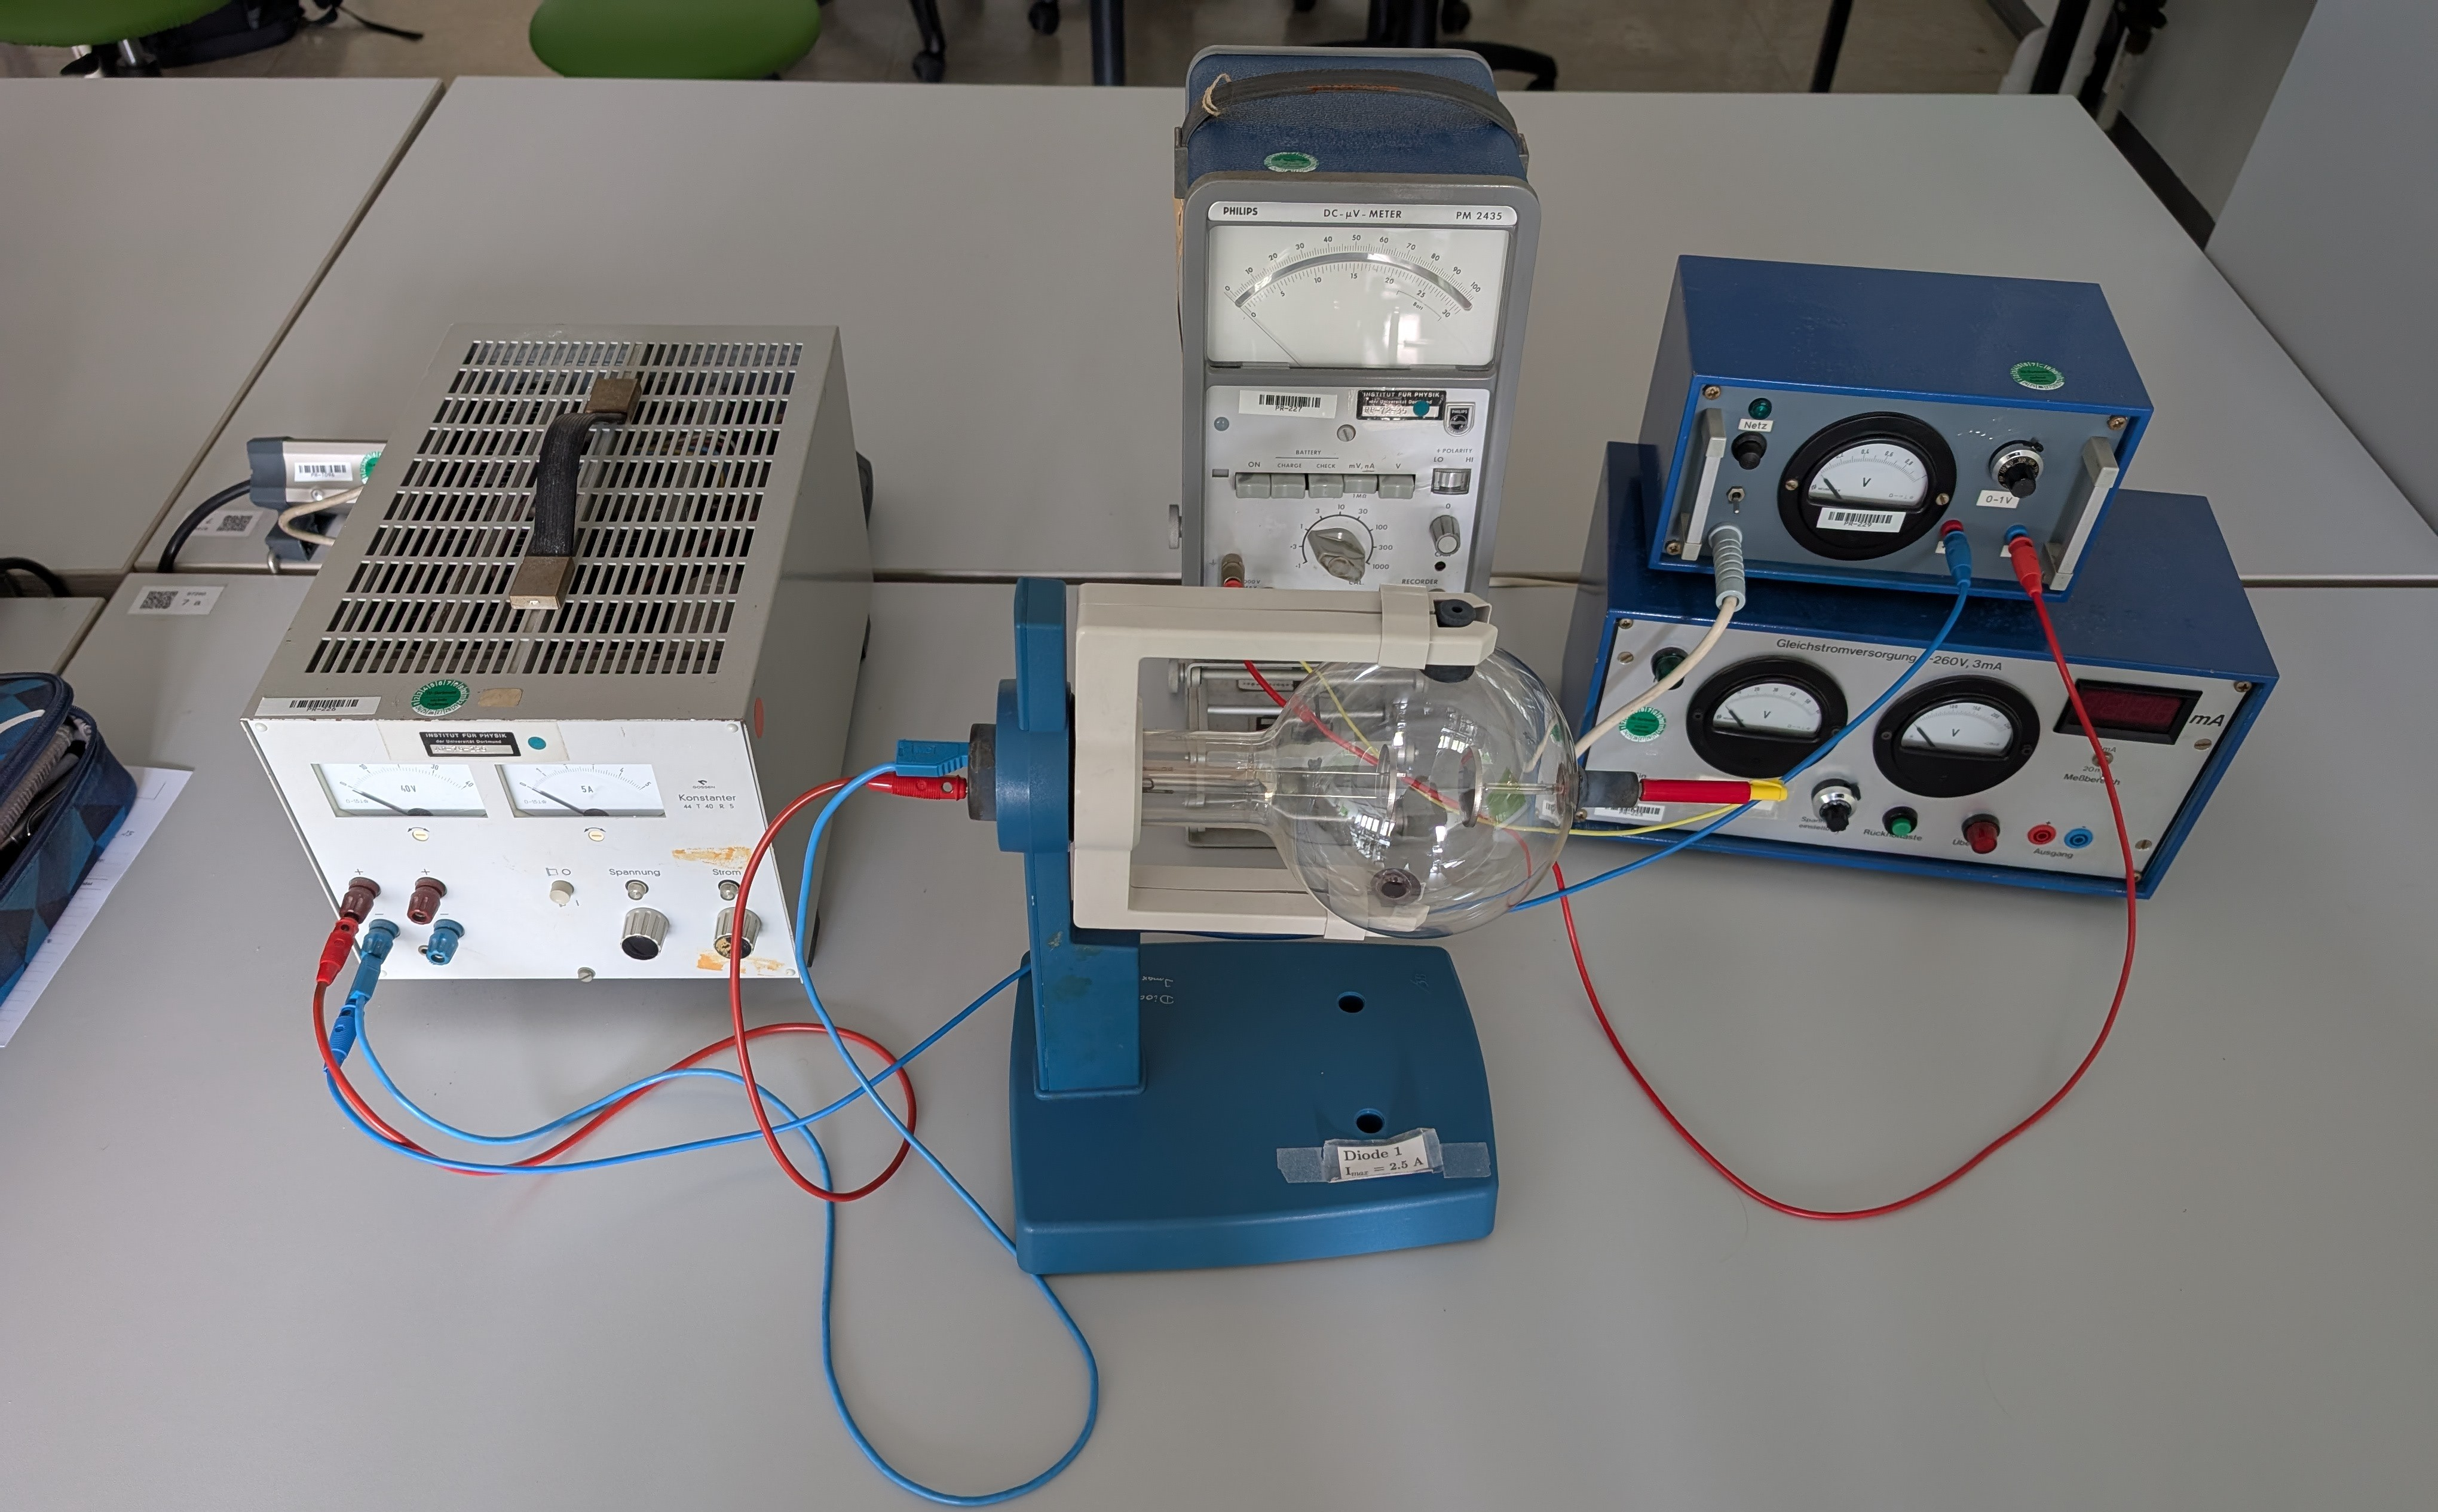
\includegraphics[width=\textwidth]{Bilder/1.jpg}
        \caption{Versuchsaufbau Anlaufstromgebiet}
    \hfill
    \label{fig:6}
\end{figure}
